\subsubsection{2.2. Kết quả kiểm thử}

\indent\indent Phần này trình bày các kết quả thực nghiệm định lượng nhằm đánh giá hiệu năng của các mô hình thực nghiệm trong đề tài. Các thang đo được sử dụng bao gồm độ chính xác (\textit{Accuracy}), độ chính xác trung bình (\textit{Macro Precision}), độ nhạy trung bình (\textit{Macro Recall}) và chỉ số F1 trung bình (\textit{Macro F1-Score}) — thước đo quan trọng nhất để đánh giá công bằng trên các tập dữ liệu mất cân bằng nhãn.\vspace{0.3cm}

\textit{2.2.1. Kết quả kiểm thử trên các mô hình GNN baseline}\vspace{0.2cm}

\textbf{Ảnh hưởng của quy mô đồ thị theo thời gian}\vspace{0.2cm}

Nhằm đánh giá độ ổn định của các kiến trúc, nghiên cứu tiến hành kiểm thử 05 mô hình Baseline trên cả 3 phạm vi dữ liệu: Tuần, Tháng và Quý. Báo cáo ghi nhận giá trị trung bình sau 5 lượt chạy độc lập, kết quả chi tiết được thể hiện tại \textbf{Bảng \ref{tab:TemporalGNN}}.

\begin{table}[H]
    \centering
    \renewcommand{\arraystretch}{1.15}
    \setlength{\tabcolsep}{5pt}
    \caption{Macro F1-Score và Accuracy của các mô hình GNN trên 3 phạm vi dữ liệu}
    \label{tab:TemporalGNN}
    \begin{tabular}{lcccccccc}
        \hline
        \multirow{2}{*}{\textbf{Mô hình}} & \multicolumn{2}{c}{\textbf{Phạm vi Tuần}} & \multicolumn{2}{c}{\textbf{Phạm vi Tháng}} & \multicolumn{2}{c}{\textbf{Phạm vi Quý}} & \multicolumn{2}{c}{\textbf{Trung bình chung}} \\ \cline{2-9} 
        & \textbf{Acc} & \textbf{F1} & \textbf{Acc} & \textbf{F1} & \textbf{Acc} & \textbf{F1} & \textbf{Acc} & \textbf{F1} \\ 
        \hline
        GCN                  & \textbf{1.0000} & \textbf{1.0000} & 0.9113 & 0.8743 & 0.8530 & 0.8019 & 0.9214 & 0.8921 \\
        GINE                 & 0.9400 & 0.9314 & 0.7599 & 0.6807 & 0.7222 & 0.6650 & 0.8074 & 0.7590 \\
        PNA                  & 0.9733 & 0.9712 & 0.9113 & 0.8719 & 0.8756 & 0.8085 & 0.9201 & 0.8839 \\
        \textbf{GATv2}       & 0.9800 & 0.9865 & \textbf{0.9338} & \textbf{0.9033} & 0.9062 & 0.8655 & \textbf{0.9400} & \textbf{0.9184} \\
        Transformer          & 0.9800 & 0.9804 & 0.9070 & 0.8637 & \textbf{0.9074} & \textbf{0.8683} & 0.9315 & 0.9041 \\
        \hline
    \end{tabular}
\end{table}

Kết quả thực nghiệm chỉ ra một xu hướng quan trọng: Hiệu năng của tất cả các mô hình đều rất cao trên tập Tuần (thậm chí GCN đạt mức tuyệt đối), nhưng suy giảm dần khi mở rộng sang tập Tháng và Quý. Điều này phản ánh chính xác bản chất phức tạp của đồ thị mạng xã hội phi tập trung. Ở quy mô Tuần, số lượng nút ít, cấu trúc của các cụm Sybil bộc lộ rất thô sơ và dễ bị phát hiện. Tuy nhiên, ở phạm vi Quý, đồ thị trở nên khổng lồ với hàng trăm nghìn liên kết đan chéo, kết hợp với các chiến thuật ngụy trang tinh vi của Sybil, khiến ranh giới phân lớp bị mờ đi.\vspace{0.3cm}

Bất chấp độ khó của tập dữ liệu Quý, các mô hình có cơ chế chú ý là \textbf{GATv2} và \textbf{Transformer} vẫn thể hiện sự bền bỉ vượt trội, duy trì mức Macro F1 trên 0.86 và trở thành hai ứng cử viên sáng giá nhất.\vspace{0.3cm}

\textbf{Phân tích sâu trên phạm vi Quý}\vspace{0.2cm}

\indent Vì tập dữ liệu Quý mang tính đại diện cao nhất cho môi trường thực tế, đánh giá chi tiết được thực hiện chuyên sâu trên tập dữ liệu này. \textbf{Bảng \ref{tab:QuarterDetail}} thống kê các chỉ số hiệu năng cụ thể của 05 mô hình.

\begin{table}[H]
    \centering
    \renewcommand{\arraystretch}{1.0}
    \caption{Hiệu năng phân loại của các mô hình GNN Baseline trên phạm vi Quý}
    \label{tab:QuarterDetail}
    \begin{tabular}{lccccc}
        \hline
        \textbf{Mô hình} & \textbf{Test Loss} & \textbf{Accuracy} & \textbf{Macro Precision} & \textbf{Macro Recall} & \textbf{Macro F1} \\
        \hline
        GCN                  & 0.6373 & 0.8530 & 0.7791 & 0.8359 & 0.8019 \\
        GINE                 & 0.5580 & 0.7222 & 0.6728 & 0.7691 & 0.6650 \\
        PNA                  & 0.6208 & 0.8756 & 0.7895 & 0.8379 & 0.8085 \\
        \textbf{GATv2}       & \textbf{0.3860} & 0.9062 & 0.8416 & \textbf{0.8969} & 0.8655 \\
        \textbf{Transformer} & 0.8647 & \textbf{0.9074} & \textbf{0.8531} & 0.8859 & \textbf{0.8683} \\
        \hline
    \end{tabular}
\end{table}

Dựa trên kết quả, ta có thể đánh giá năng lực của từng kiến trúc:
\begin{itemize}[label={--}, itemsep=1pt]
    \item \textbf{Nhóm GATv2 và Transformer:} Dẫn đầu bảng xếp hạng với Macro F1 bám sát nhau (tương ứng 0.8655 và 0.8683). Mặc dù Transformer nhỉnh hơn một chút về F1, nhưng GATv2 lại sở hữu mức Test Loss thấp nhất toàn dải (0.3860) so với mức rất cao của Transformer (0.8647). Điều này chứng minh GATv2 là mô hình có độ tin cậy (\textit{confidence}) cao nhất và tối ưu hóa tốt nhất.
    \item \textbf{Nhóm GCN và PNA:} Đạt hiệu năng ở mức khá (Macro F1 $\approx 0.80$). Việc GCN sử dụng ma trận bậc tĩnh khiến nó mất đi khả năng nhận diện các Sybil tinh vi.
    \item \textbf{GINE:} Thể hiện kết quả kém nhất (Macro F1: 0.6650). Mặc dù có tính biểu diễn lý thuyết mạnh, kiến trúc quá phức tạp của GINE dễ dẫn đến hiện tượng nhiễu thông tin trên các đồ thị có mật độ cạnh lớn trong bài toán hiện tại
\end{itemize}

\textbf{Đánh giá năng lực phân loại qua đường cong ROC}\vspace{0.2cm}

\indent Bên cạnh các chỉ số điểm danh định, nghiên cứu thực hiện đánh giá khả năng phân tách giữa các nhóm đối tượng ở nhiều ngưỡng xác suất thông qua biểu đồ đường cong ROC. Do đặc thù phân loại 4 lớp, đường cong ROC được tổng hợp bằng phương pháp \textbf{Macro-average} (trung bình cộng One-vs-Rest của cả 4 nhãn).

\begin{figure}[H]
    \centering
    \fbox{\includegraphics[width=0.65\linewidth]{images/part-02/chap-03/sec-02/ROCBaselineQuarter.png}}
    \vspace{0.1cm}
    \caption{So sánh đường cong ROC của các kiến trúc GNN Baseline trên phạm vi Quý}
    \label{fig:ROC_Baseline}
\end{figure}

Từ kết quả trực quan tại \textbf{Hình \ref{fig:ROC_Baseline}}, GATv2 (và Transformer) tiếp tục khẳng định sự vượt trội khi đường cong áp sát về góc trên cùng bên trái, đạt chỉ số AUC cao nhất. Mô hình duy trì được tỷ lệ Dương tính thật (\textit{TPR}) ở mức cao trong khi vẫn kiểm soát nghiêm ngặt tỷ lệ Dương tính giả (\textit{FPR}). Biểu đồ ROC một lần nữa tái khẳng định quyết định lựa chọn \textbf{GATv2} làm bộ trích xuất đặc trưng xương sống cho kiến trúc phân lớp tách rời là hoàn toàn có cơ sở khoa học.\vspace{0.3cm}

\textit{2.2.2. Kết quả kiểm thử trên kiến trúc phân lớp tách rời (Decoupled GNN-ML)}\vspace{0.2cm}

\textbf{Đánh giá tổng quan các tổ hợp kiến trúc}\vspace{0.2cm}

Kiến trúc Decoupled tận dụng các mô hình GNN đã được đóng băng trọng số làm bộ trích xuất đặc trưng. Các vector nhúng 16 chiều sau đó được đưa vào 04 thuật toán học máy truyền thống để phân loại. Để đánh giá toàn diện 20 tổ hợp (5 GNN $\times$ 4 ML), nghiên cứu sử dụng biểu đồ nhiệt thể hiện hai chỉ số quan trọng nhất: \textit{Macro F1-Score} và \textit{Accuracy} trung bình.

\begin{figure}[H]
    \centering
    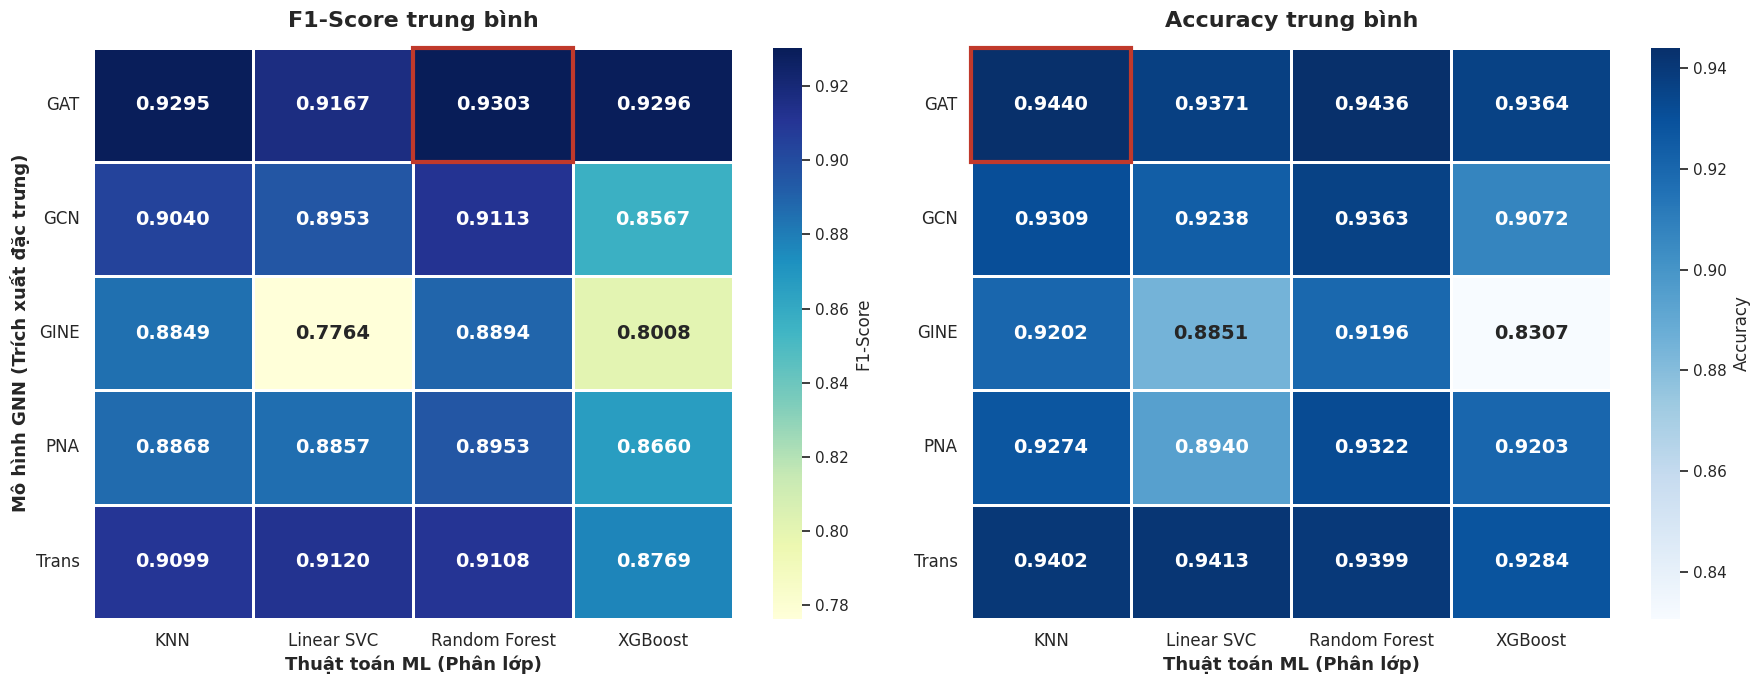
\includegraphics[width=\linewidth]{images/part-02/chap-03/sec-02/GNN-MLHeatmapComparison.png}
    \vspace{0.1cm}
    \caption{Ma trận hiệu năng chéo của các tổ hợp Decoupled GNN-ML}
    \label{fig:DecoupledHeatmap}
\end{figure}

Từ \textbf{Hình \ref{fig:DecoupledHeatmap}}, có thể rút ra những phân tích sâu sắc về sự tương thích giữa không gian nhúng đồ thị và các không gian phân lớp:

\begin{itemize}[label={--}, itemsep=1pt]
    \item \textbf{Sự thống trị của GATv2 Backbone:} Điều này một lần nữa khẳng định cơ chế \textit{Attention} của GATv2 đã nén thông tin từ không gian 396 chiều ban đầu xuống 16 chiều một cách xuất sắc, giữ lại được những ranh giới phân tách rõ ràng nhất giữa tài khoản Sybil và tài khoản thật.
    \item \textbf{Khả năng tương thích của Random Forest và KNN:} Nhìn theo trục ngang, các thuật toán phi tuyến tính như \textbf{Random Forest} và dựa trên khoảng cách như \textbf{KNN} hoạt động cực kỳ hiệu quả trên dữ liệu nhúng của đồ thị. Đặc biệt, tổ hợp vô địch toàn cục gọi tên \textbf{GATv2 + Random Forest} với \textit{Macro F1} đạt \textbf{0.9303} và \textit{Accuracy} đạt \textbf{0.9436}. Việc sử dụng quần thể cây quyết định giúp Random Forest phân tách tốt các biên giới phức tạp mà GATv2 đã tạo ra trong không gian tiềm ẩn.
    \item \textbf{Sự sụt giảm của LinearSVC:} Mô hình phân loại tuyến tính (LinearSVC) nhìn chung cho kết quả thấp nhất (đặc biệt khi kết hợp với GINE, F1 chỉ đạt 0.7764). Điều này chứng minh rằng các cụm hành vi Sybil trong không gian tiềm ẩn không phân bố tuyến tính, đòi hỏi các ranh giới quyết định phức tạp hơn.
\end{itemize}

\textbf{So sánh hiệu năng với Baseline qua các phạm vi thời gian}\vspace{0.2cm}

Để khẳng định tính ổn định và khả năng mở rộng của phương pháp đề xuất, nghiên cứu tiến hành so sánh trực diện giữa mô hình Baseline tốt nhất (\textbf{GATv2}) và tổ hợp Decoupled xuất sắc nhất (\textbf{GATv2 + Random Forest}) trên cả 3 phạm vi thời gian. Các chỉ số được trình bày chi tiết tại \textbf{Bảng \ref{tab:HeadToHead}}.

\begin{table}[H]
    \centering
    \renewcommand{\arraystretch}{1.15}
    \setlength{\tabcolsep}{4.5pt}
    \caption{So sánh hiệu năng GATv2 Baseline và GATv2 + RF}
    \label{tab:HeadToHead}
    \begin{tabular}{lcccccccc}
        \hline
        \multirow{2}{*}{\textbf{Kiến trúc mô hình}} & \multicolumn{2}{c}{\textbf{Phạm vi Tuần}} & \multicolumn{2}{c}{\textbf{Phạm vi Tháng}} & \multicolumn{2}{c}{\textbf{Phạm vi Quý}} & \multicolumn{2}{c}{\textbf{Trung bình chung}} \\ \cline{2-9} 
        & \textbf{Acc} & \textbf{F1} & \textbf{Acc} & \textbf{F1} & \textbf{Acc} & \textbf{F1} & \textbf{Acc} & \textbf{F1} \\ 
        \hline
        GATv2 (Baseline) & \textbf{0.9800} & \textbf{0.9865} & 0.9338 & 0.9033 & 0.9062 & 0.8655 & 0.9400 & 0.9184 \\
        \textbf{GATv2 + Random Forest} & 0.9667 & 0.9776 & \textbf{0.9472} & \textbf{0.9299} & \textbf{0.9170} & \textbf{0.8833} & \textbf{0.9436} & \textbf{0.9303} \\
        \hline
    \end{tabular}
\end{table}

Dữ liệu thực nghiệm từ \textbf{Bảng \ref{tab:HeadToHead}} bộc lộ một xu hướng dịch chuyển hiệu năng vô cùng đáng chú ý liên quan đến quy mô của đồ thị:

\begin{itemize}[label={--}, itemsep=1pt]
    \item \textbf{Hiện tượng tại phạm vi Tuần (Đồ thị quy mô nhỏ):} Mô hình GATv2 baseline đạt kết quả nhỉnh hơn (Macro F1 đạt 0.9865 so với 0.9776 của tổ hợp). Nguyên nhân là do ở phạm vi Tuần, cấu trúc đồ thị còn tương đối thưa thớt, các hành vi của các cụm Sybil có ranh giới rất rõ ràng. Một mạng nơ-ron sâu như GATv2 dễ dàng "học thuộc" và phân tách hoàn hảo các đặc trưng này.
    \item \textbf{Sự bứt phá tại phạm vi Tháng và Quý (Đồ thị quy mô lớn):} Khi đồ thị mở rộng, lượng nhiễu tăng đột biến do các tài khoản Sybil chủ động tăng cường tương tác chéo để ngụy trang. Tại đây, hiệu năng của GATv2 thuần bắt đầu suy giảm nhanh (F1 từ 0.9865 xuống 0.8655). Ngược lại, tổ hợp \textbf{GATv2 + Random Forest} chứng minh được sự bền bỉ đáng kinh ngạc, vượt lên dẫn trước với khoảng cách an toàn (F1 đạt 0.8833 trên tập Quý). 
    \item \textbf{Lý giải nguyên nhân:} Sự vượt trội của tổ hợp Decoupled trên đồ thị lớn đến từ bản chất của thuật toán \textit{Random Forest}. Quần thể các cây quyết định có khả năng chống nhiễu cực kỳ mạnh mẽ. Khi GATv2 đã hoàn thành nhiệm vụ và cho ra các vector embedding 16 chiều, Random Forest chỉ tập trung thiết lập các ranh giới phi tuyến tính mà không bị ảnh hưởng bởi các vấn đề truyền tải thông điệp trên đồ thị lớn.
\end{itemize}

Việc tách rời trích xuất đặc trưng và phân lớp trực tiếp nâng cao độ ổn định của mô hình khi đối mặt với các đồ thị mạng xã hội phi tập trung có mật độ dày đặc trong thực tế.\vspace{0.3cm}

\textbf{Phân tích chuyên sâu mô hình vô địch (GATv2 + Random Forest)}\vspace{0.2cm}

Các chỉ số trung bình tuy cung cấp cái nhìn tổng quan về hiệu năng, nhưng không phản ánh được năng lực thực sự của mô hình trên từng nhóm đối tượng cụ thể. Đặc biệt, trong bài toán phát hiện Sybil, việc nhận diện chính xác nhóm \textit{Malicious} mang tính sống còn, trong khi việc không nhận diện nhầm nhóm \textit{Benign} giúp đảm bảo an toàn cho người dùng thật. Vì vậy, đánh giá chuyên sâu được thực hiện trên tổ hợp tốt nhất (GATv2 + Random Forest) tại phạm vi Quý.

\begin{table}[H]
    \centering
    \renewcommand{\arraystretch}{1.2}
    \setlength{\tabcolsep}{10pt}
    \caption{Báo cáo phân loại chi tiết của GATv2 + Random Forest trên phạm vi Quý}
    \label{tab:ClassReportRF}
    \begin{tabular}{lcccc}
        \hline
        \textbf{Lớp} & \textbf{Precision} & \textbf{Recall} & \textbf{F1-Score} & \textbf{Support} \\
        \hline
        BENIGN        & 0.9331 & 0.9208 & 0.9269 & 303 \\
        LOW\_RISK     & 0.7479 & 0.8018 & 0.7739 & 111 \\
        HIGH\_RISK    & 0.9574 & 0.9464 & 0.9518 & 522 \\
        MALICIOUS     & 0.8788 & 0.9062 & 0.8923 & 64 \\
        \hline
        \textbf{Accuracy}          & & & \textbf{0.9200} & 1000 \\
        \textbf{Macro avg}         & 0.8793 & 0.8938 & 0.8862 & 1000 \\
        \textbf{Weighted avg}      & 0.9217 & 0.9200 & 0.9207 & 1000 \\
        \hline
    \end{tabular}
\end{table}

Để có cái nhìn trực quan hơn về phân phối lỗi dự đoán và các điểm mù của kiến trúc, nghiên cứu tiến hành xây dựng Ma trận nhầm lẫn như thể hiện tại \textbf{Hình \ref{fig:CMRandomForest}}.

\begin{figure}[H]
    \centering
    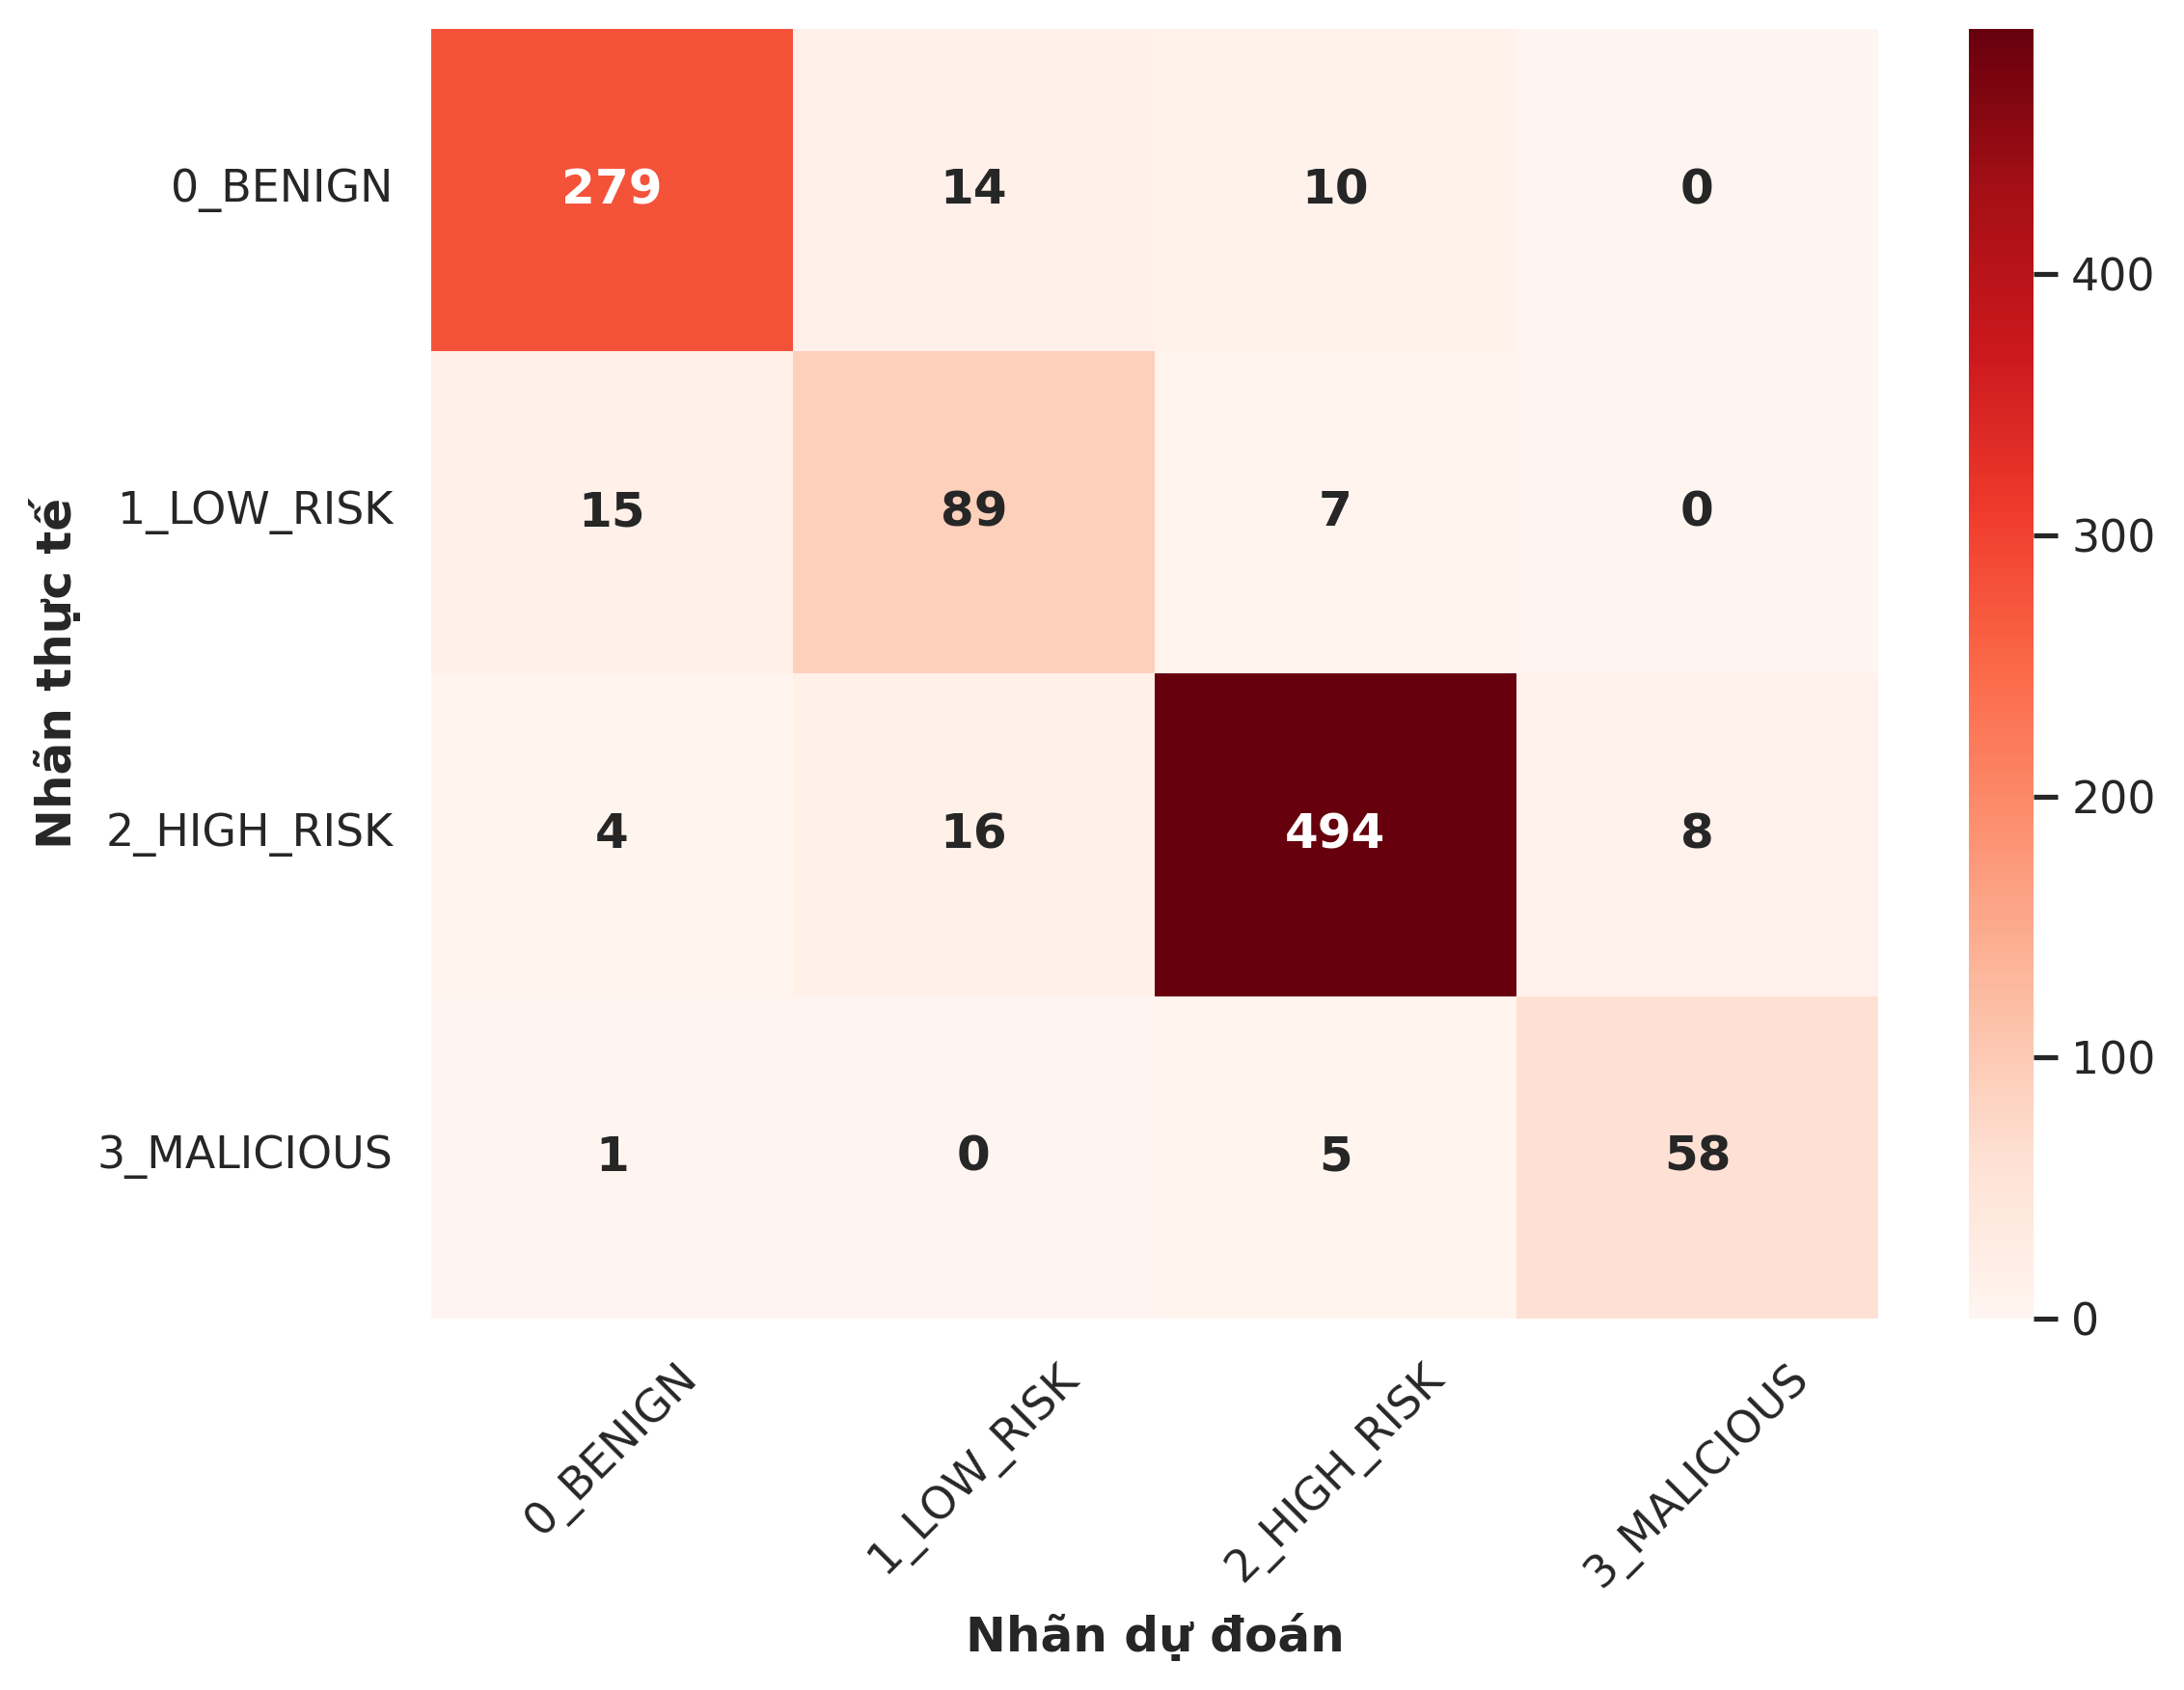
\includegraphics[width=0.65\linewidth]{images/part-02/chap-03/sec-02/CMGATv2RFQuarter.png}
    \vspace{0.1cm}
    \caption{Ma trận nhầm lẫn của GATv2 + Random Forest (Phạm vi Quý)}
    \label{fig:CMRandomForest}
\end{figure}

Từ báo cáo phân loại và ma trận nhầm lẫn, có thể rút ra những nhận định chuyên sâu về độ tin cậy của mô hình đề xuất:
\begin{itemize}[label={--}, itemsep=1pt]
    \item \textbf{Bảo vệ người dùng thật (Benign):} Mô hình đạt F1-Score lên tới 0.9269 cho nhóm người dùng bình thường. Quan trọng nhất, quan sát trên ma trận nhầm lẫn cho thấy trong số 303 tài khoản \textit{Benign}, không có bất kỳ tài khoản nào bị mô hình gán nhầm thành \textit{Malicious}. Điều này chứng minh hệ thống cực kỳ an toàn để triển khai thực tế, tránh được rủi ro khóa nhầm tài khoản gây thiệt hại nghiêm trọng.
    \item \textbf{Độ nhạy bắt Sybil xuất sắc (Malicious):} Chỉ số \textit{Recall} của nhóm Malicious đạt 0.9062 (phát hiện thành công 58/64 Sybil thực sự). Việc chỉ bỏ lọt 1 tài khoản Sybil sang nhóm Benign cho thấy thuật toán Random Forest kết hợp với đặc trưng Attention đã bóc tách được gần như toàn bộ các mạng lưới bầy đàn, kể cả những nhóm ngụy trang tinh vi nhất trong đồ thị Quý.
    \item \textbf{Sự nhầm lẫn tự nhiên:} Phần lớn lỗi của hệ thống tập trung ở việc nhầm lẫn giữa \textit{High Risk} và \textit{Malicious} (8 mẫu High Risk bị đoán là Malicious, và 5 mẫu Malicious bị đoán là High Risk). Trên phương diện phân tích dữ liệu Web3, đây là một hiện tượng chấp nhận được và mang tính bản chất.
\end{itemize}